\section{Objective-Specific Checks}
\label{app:results-details}
\subsection{O1: Partial ownership and regression robustness}
\label{app:results-o1}
\begin{mergedcontribution}{authorSowmya}
\subsubsection{O1: Concentration and regression}
\label{app:o1-definitions}
\label{app:o1-dictionary}
Common measures follow Appendix~\ref{app:shared-calculations}. The grouping effect is Ownership-HHI minus Brand-HHI; the partial-ownership effect is MHHI minus Ownership-HHI; their sum is MHHI minus Brand-HHI. The IndiGo ratio divides its share by the second-largest group's. Event indicators and trends explain the index outcomes; COVID and seasonal indicators are controls. MHHI uses proportional control unless stated otherwise.

\subsubsection{National input tables}
\label{app:eda-national-inputs}
Table~\ref{tab:o1-periods} groups the monthly observations into four periods, separated by the Jet Airways exit in April 2019, Tata's acquisition of Air India in January 2022 and the late-2024 mergers. These are period means rather than individual monthly observations.

\begin{minipage}{\linewidth}
\captionsetup{font={small,color=authorSowmya},labelfont=bf,justification=raggedright,singlelinecheck=false,hypcap=false}
\captionof{table}{O1: Concentration measures by period (period means).}
\label{tab:o1-periods}
\centering
{\small\setstretch{1.1}\setlength{\tabcolsep}{4pt}
\fontsize{10}{12}\selectfont\setstretch{1}\setlength{\tabcolsep}{3pt}
\renewcommand{\arraystretch}{1.15}
\begin{tabular}{|>{\raggedright\arraybackslash}p{\dimexpr0.28\linewidth-2\tabcolsep-1.1428571428571428\arrayrulewidth\relax}|>{\raggedright\arraybackslash}p{\dimexpr0.12\linewidth-2\tabcolsep-1.1428571428571428\arrayrulewidth\relax}|>{\raggedright\arraybackslash}p{\dimexpr0.12\linewidth-2\tabcolsep-1.1428571428571428\arrayrulewidth\relax}|>{\raggedright\arraybackslash}p{\dimexpr0.12\linewidth-2\tabcolsep-1.1428571428571428\arrayrulewidth\relax}|>{\raggedright\arraybackslash}p{\dimexpr0.12\linewidth-2\tabcolsep-1.1428571428571428\arrayrulewidth\relax}|>{\raggedright\arraybackslash}p{\dimexpr0.12\linewidth-2\tabcolsep-1.1428571428571428\arrayrulewidth\relax}|>{\raggedright\arraybackslash}p{\dimexpr0.12\linewidth-2\tabcolsep-1.1428571428571428\arrayrulewidth\relax}|}
\hline
\textbf{Period} & \textbf{Brand HHI} & \textbf{Own.\ HHI} & \textbf{MHHI} & \textbf{CR2 (\%)} & \textbf{Gap (pp)} & \textbf{Fringe (\%)} \\
\hline
Pre-Jet exit (Jan 2015--Apr 2019) & 2{,}323.8 & 2{,}408.0 & 2{,}416.1 & 58.7 & 21.8 & 41.3 \\
\hline
Jet exit to Tata (May 2019--Dec 2021) & 3{,}293.1 & 3{,}294.5 & 3{,}342.3 & 66.9 & 39.2 & 33.1 \\
\hline
Tata to mergers (Jan 2022--Nov 2024) & 3{,}847.6 & 4{,}308.6 & 4{,}308.6 & 85.5 & 33.1 & 14.5 \\
\hline
Post mergers (Dec 2024--Jul 2026) & 4{,}538.0 & 4{,}876.7 & 4{,}876.7 & 90.7 & 38.0 & 9.3 \\
\hline
\end{tabular}\par}
\vspace{4pt}
{\footnotesize\setstretch{1.1}\raggedright\textit{Note:} HHI values are index points; CR2, gap and fringe use ownership-group passenger shares. April 2020 is missing and not imputed.\par
\textit{Source:} DGCA monthly airline traffic via \href{https://github.com/mkubicek/india-aviation-stats/tree/16770ac59dae61ce7b80fd8bd67dd7f4cef280a6}{Kubicek (2026)}; authors' calculations.\par}
\end{minipage}

\subsubsection{Cleaning and sensitivity checks}
\label{app:o1-cleaning}
The cleaning excludes 1,773 out-of-scope rows and 132 zero-passenger rows; there are no missing key fields or duplicate airline-months. Names are standardised, but the January 2024 AIX Connect rebrand is retained. Observed counts are never overwritten. Shares close to 100\% in all 138 observed months. Two positive-passenger records have zero ASK/RPK (Air Odisha, September 2018; Air Deccan, March 2020); they remain flagged, not imputed.

The $|\Delta\ln q|>0.7$ screen finds 92 flags: 45 COVID/market-wide, 23 entry/exit, one merger and 23 unexplained but immaterial ($<1\%$ share); none is material. Dropping the latter changes Brand-HHI by at most 70.6 points and Ownership-HHI/MHHI by 34.5. Of 12 within-spell missing runs, AirAsia India's January--December 2017 gap is material (bracketing share 3.6\%; HHI overstatement about 165--171 points). Only sensitivity runs interpolate it. Missing April 2020 and Go First's May 2020 lockdown suspension are not imputed.

\subsubsection{O1: MHHI algorithm and stake schedule}
\label{app:o1-stakes}
For each market-month: (S1) compute brand shares and Brand-HHI; (S2) map brands to ownership groups by date, sum to $S_{gt}$, and compute Ownership-HHI, CR2 and the effective number of firms; (S3) load each owner's stake $\beta_{ik}$ from Table~\ref{tab:o1-stakes}; (S4) set control $\gamma_{ik}=\beta_{ik}$ (proportional) or $\gamma=1$ for a majority owner; (S5) compute $\lambda_{jk}$ and MHHI from Equation~O1.1b. Only the stakes in the table are modelled; a firm with no listed stake is wholly owned.

\begin{minipage}{\linewidth}
\captionsetup{font={small,color=authorSowmya},labelfont=bf,justification=raggedright,singlelinecheck=false,hypcap=false}
\captionof{table}{O1: Partial-ownership schedule used for MHHI (financial stakes $\beta$).}
\label{tab:o1-stakes}
\centering
{\footnotesize\setstretch{1.0}\setlength{\tabcolsep}{4pt}
\fontsize{10}{12}\selectfont\setstretch{1}\setlength{\tabcolsep}{3pt}
\renewcommand{\arraystretch}{1.15}
\begin{tabular}{|l|l|r|r|r|c|}
\hline
\textbf{Firm} & \textbf{Months applied} & \textbf{Tata} & \textbf{Partner} & \textbf{Other} & \textbf{Source} \\
\hline
Vistara & Jan 2015--Dec 2021 & 51 & 49 & -- & a \\
\hline
AirAsia India & Jan--Aug 2015 & 30 & 49 & 21 & b \\
\hline
AirAsia India & Sep 2015--Mar 2016 & 41.06 & 49 & 9.94 & c \\
\hline
AirAsia India & Apr 2016--Dec 2019 & 49 & 49 & 2 & c, d \\
\hline
AirAsia India & Jan--Dec 2020 & 51 & 49 & -- & e \\
\hline
AirAsia India & Jan--Dec 2021 & 83.67 & 16.33 & -- & e, f \\
\hline
\end{tabular}\par}
\vspace{4pt}
{\footnotesize\setstretch{1.0}\raggedright\textit{Note:} Stakes are percentages. Partner means Singapore Airlines (Vistara) or AirAsia Investment; other means Telestra through March 2016, then two individuals. Dashes mean no other stake. Sources: (a) \textcite{sia2015annual,sia2022merger}; (b) \textcite{airasia2013jv}; (c) \textcite{tata2016airasia}; (d) \textcite{airasia2018q4}; (e) \textcite{airasia2021disposal}; (f) \textcite{airasia2021results}. Changes apply from the next month. The undated 49-to-51\% step is placed in January 2020; using April 2016 changes the pre-2022 mean wedge from 22.9 to 23.1. Foreign partners hold no other Indian airline stake: they enter only $\lambda$'s denominator. Unlisted firms are wholly owned.\par}
\end{minipage}

Interpolating AirAsia India's missing 2017 records raises the pre-2022 mean partial-ownership adjustment from 22.9 to 24.9 points. Treating Tata's 51\% stake in Vistara as full control raises it to 36.9 points, with a maximum of 119.6. These are sensitivity checks, rather than changes to the headline grouping convention.

\subsubsection{Regression robustness and diagnostics}
\label{app:o1-cr2}
\label{app:o1-robust}
Table~\ref{tab:o1-robust} combines the lag, COVID and missing-data checks with CR2 event coefficients. Re-dating Jet and Go First steps to the drifts gives Ownership-HHI steps 396, 933, 696 and 186 (sum 2,211; $R^2=0.985$); Brand-HHI and MHHI sums are 1,801 and 2,162, all steps significant at 1\%.

\begin{minipage}{\linewidth}
\captionsetup{font={small,color=authorSowmya},labelfont=bf,justification=raggedright,singlelinecheck=false,hypcap=false}
\captionof{table}{O1: Ownership-HHI robustness and CR2 event checks.}
\label{tab:o1-robust}
\label{tab:o1-cr2reg}
\label{tab:detail-o1-regression}
\centering
{\small\setstretch{1.1}\setlength{\tabcolsep}{5pt}
\fontsize{10}{12}\selectfont\setstretch{1}\setlength{\tabcolsep}{3pt}
\renewcommand{\arraystretch}{1.15}
\begin{tabular}{|>{\raggedright\arraybackslash}p{\dimexpr0.44\linewidth-2\tabcolsep-1.2\arrayrulewidth\relax}|>{\raggedright\arraybackslash}p{\dimexpr0.14\linewidth-2\tabcolsep-1.2\arrayrulewidth\relax}|>{\raggedright\arraybackslash}p{\dimexpr0.14\linewidth-2\tabcolsep-1.2\arrayrulewidth\relax}|>{\raggedright\arraybackslash}p{\dimexpr0.14\linewidth-2\tabcolsep-1.2\arrayrulewidth\relax}|>{\raggedright\arraybackslash}p{\dimexpr0.14\linewidth-2\tabcolsep-1.2\arrayrulewidth\relax}|}
\hline
\textbf{Specification} & \textbf{Jet exit} & \textbf{Tata} & \textbf{Go First} & \textbf{Mergers} \\
\hline
Baseline (Newey--West 12 lags) & 312 (3.9) & 900 (10.8) & 640 (11.4) & 137 (2.5) \\
\hline
Newey--West 6 lags & 312 (3.8) & 900 (9.8) & 640 (10.4) & 137 (2.2) \\
\hline
Newey--West 18 lags & 312 (4.6) & 900 (12.1) & 640 (12.0) & 137 (2.8) \\
\hline
COVID months dropped & 330 (4.6) & 899 (10.6) & 656 (12.0) & 136 (2.5) \\
\hline
AirAsia India 2017 interpolated & 371 (4.0) & 920 (10.0) & 652 (10.6) & 148 (2.6) \\
\hline
\multicolumn{5}{|l|}{CR2 event steps in pp, with Newey--West (12-lag) standard errors} \\
\hline
Ownership-group CR2 & 5.72 (0.95) & 17.95 (1.18) & 9.29 (1.31) & 1.41 (0.58) \\
\hline
Brand CR2 & 6.95 (1.07) & 1.90 (0.92) & 6.47 (0.76) & 6.53 (0.74) \\
\hline
\end{tabular}\par}
{\footnotesize\raggedright HHI rows show coefficients and $t$-statistics; CR2 rows show coefficients and standard errors. CR2 step sums are 34.4 (2.6) and 21.9 (2.8), group/brand respectively; trends $-0.02$ (0.02) and 0.01 (0.03); COVID 5.03 (0.73) and 4.44 (0.77); $R^2$ 0.984/0.958; Durbin--Watson 0.80/0.84. For the main Brand-HHI, Ownership-HHI and MHHI regressions, Durbin--Watson is 0.92/0.93/0.94. Breusch--Godfrey (12 lags) rejects no autocorrelation and ADF rejects a residual unit root in all five models ($p<0.001$); inference uses Newey--West errors. Source: authors' calculations.\par}
\end{minipage}
\vspace{0.8em}

\subsubsection{O1: Formulae and model specification}
\label{app:review-o1-formulae}
Let $q_{it}$ be brand $i$'s domestic passengers in month $t$. Its percentage share and the share of ownership group $g$ are
\[
s_{it}=100\frac{q_{it}}{\sum_j q_{jt}},\qquad S_{gt}=\sum_{i\in g}s_{it}.
\]
Air India and Air India Express form one group, as do Jet Airways and JetLite. Vistara and AirAsia India/AIX Connect join the Air India Group from January 2022 under the study's grouping convention. The three indices and the regression model are defined as follows:
\begin{align}
\text{Brand-HHI}_t &= \sum_i s_{it}^2, \qquad \text{Ownership-HHI}_t = \sum_g S_{gt}^2 \tag{O1.1a}\label{eq:review-o1-indices}\\
\text{MHHI}_t &= \text{Ownership-HHI}_t+\sum_{j}\sum_{k\neq j}\lambda_{jk}S_{jt}S_{kt},\qquad
\lambda_{jk}=\frac{\sum_i \gamma_{ij}\beta_{ik}}{\sum_i \gamma_{ij}\beta_{ij}} \tag{O1.1b}\label{eq:review-o1-mhhi}
\end{align}
Here $\beta_{ik}$ is owner $i$'s stake in firm $k$ and $\gamma_{ik}$ its control share \parencite{obriensalop2000}. The regression is
\begin{equation}
\text{Index}_t = \alpha + \beta t + \sum_{k=1}^{4}\gamma_k\,\text{Post}_{kt} + \delta\,\text{COVID}_t + \sum_{m=2}^{12}\mu_m M_{mt} + \varepsilon_t \tag{O1.2}\label{eq:review-o1-regression}
\end{equation}
Here $\beta$ is the monthly trend, $\gamma_k$ the event coefficients, $\delta$ the COVID coefficient and $\mu_m$ the seasonal coefficients, with January as the base month. Each post-event indicator is zero before its date and one thereafter. The dates and COVID window are given in Section~\ref{sec:method-o1} (O1). Newey--West standard errors use 12 lags \parencite{neweywest1987}. These are descriptive shifts, not causal effects; robustness checks are in Appendix~\ref{app:o1-robust}.

Other measures are
\[
\mathrm{CR2}_t=S_{(1)t}+S_{(2)t},\qquad
N_{\mathrm{effective},t}=\frac{10{,}000}{\mathrm{Ownership\mbox{-}HHI}_t}.
\]
The two ownership comparisons are
\begin{align*}
\mathrm{Grouping\ effect}_t&=\mathrm{Ownership\mbox{-}HHI}_t-\mathrm{Brand\mbox{-}HHI}_t,\\
\mathrm{Partial\mbox{-}ownership\ effect}_t&=\mathrm{MHHI}_t-\mathrm{Ownership\mbox{-}HHI}_t.
\end{align*}
\begin{samepage}
For each of Brand HHI, Ownership HHI and MHHI, let $x_t$ be the change from the previous available observation. The modified score is
\begingroup
\renewcommand{\theHequation}{review-o1-jump}
\begin{equation}
M_t=\frac{0.6745\,[x_t-\operatorname{median}(x)]}{\operatorname{median}|x-\operatorname{median}(x)|}.
\tag{O1.3}\label{eq:review-o1-jump}
\end{equation}
\endgroup
\par\end{samepage}
The median and median absolute deviation use all observed changes in that series \parencite{iglewicz1993outliers}. A month is flagged if $|M_t|>3.5$ in any of the three series, allowing unusually large increases and decreases. April 2020 is missing, so the May 2020 change spans March to May.

The scripts specify the seven windows D1--D7 separately from this screen. A window passes the nearby-jump check if a flagged date falls within 40 days of its end-month date. D1 and D6 do not pass this check. Window changes are the end-month index minus the start-month index. Their economic context and any subsequent reversals are assessed from the observed series.


\subsubsection{Observed and fitted concentration}

\begin{minipage}{\linewidth}
\centering
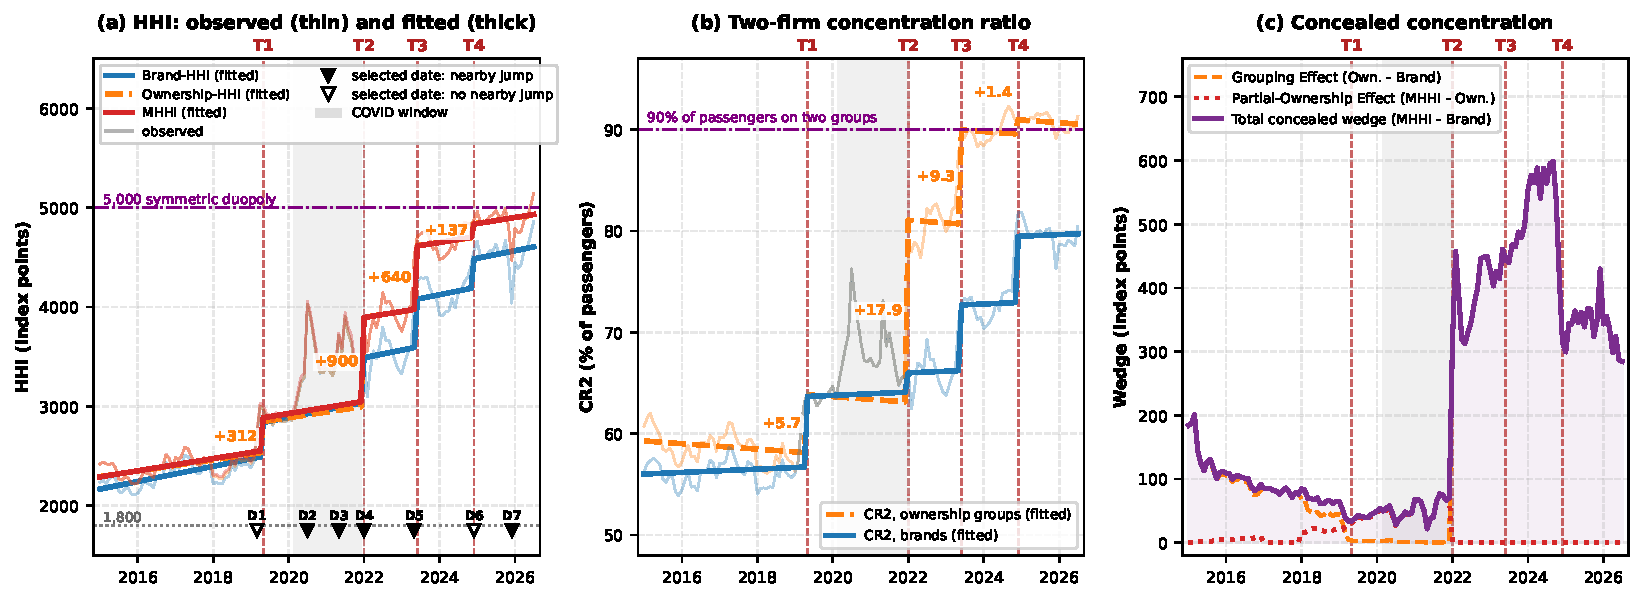
\includegraphics[width=\linewidth]{review/shortening/figures/o1_indices_review.pdf}
\captionof{figure}{O1: Interrupted time-series view of national concentration, January 2015--July 2026.}
\label{fig:o1-its}
\vspace{2pt}
\par\footnotesize\setstretch{1.1}
\textit{Note:} (a) Brand-, Ownership- and MHHI: observed (thin) and fitted (thick) values from Equation~O1.2, keeping the trend and the four event steps, with COVID and month-of-year terms netted out; figures beside each step are Ownership-HHI steps in points. (b) CR2 with its steps in percentage points. (c) Grouping Effect, Partial-Ownership Effect and their sum, the total concealed wedge. T1--T4: Jet exit, Tata acquisition, Go First exit, legal mergers. D1--D7: selected dates. Filled markers have a jump flag within 40 days; hollow markers do not. Grey band: COVID window.\par
\textit{Source:} DGCA monthly traffic via \href{https://github.com/mkubicek/india-aviation-stats/tree/16770ac59dae61ce7b80fd8bd67dd7f4cef280a6}{Kubicek (2026)}; authors' calculations.
\end{minipage}

\Needspace{4\baselineskip}
\subsubsection{Additional information for the selected windows}

\par
\begingroup
\flowtablestyle
\fontsize{10}{12}\selectfont
\begin{longtable}{|>{\raggedright\arraybackslash}p{\dimexpr0.06\linewidth-2\tabcolsep-1.25\arrayrulewidth\relax}|>{\raggedright\arraybackslash}p{\dimexpr0.19\linewidth-2\tabcolsep-1.25\arrayrulewidth\relax}|>{\raggedright\arraybackslash}p{\dimexpr0.45\linewidth-2\tabcolsep-1.25\arrayrulewidth\relax}|>{\raggedright\arraybackslash}p{\dimexpr0.3\linewidth-2\tabcolsep-1.25\arrayrulewidth\relax}|}
\caption{Share movements and coincident events for the windows in Table~\ref{tab:o1-drift}.}\label{tab:detail-o1-drift}\\
\hline
\textbf{ID} & \textbf{Window} & \textbf{Largest share movements (pp)} & \textbf{Coincident event}\\
\hline
\endfirsthead
\multicolumn{4}{c}{Table~\thetable\ (continued)}\\
\hline
\textbf{ID} & \textbf{Window} & \textbf{Largest share movements (pp)} & \textbf{Coincident event}\\
\hline
\endhead
\endfoot
\endlastfoot
D1 & Feb--Apr 2019 & Jet group $-10.4$; IndiGo $+6.4$ & Jet Airways exit\\
\hline
D2 & Jun--Jul 2020 & IndiGo $+7.6$; Air India Group $-3.3$ & Restart after the COVID lockdown\\
\hline
D3 & Apr--May 2021 & Air India Group $+6.1$; AirAsia India $-3.2$ & Second COVID wave\\
\hline
D4 & Dec 2021--Jan 2022 & Air India Group $+13.9$ (Vistara $-7.7$, AirAsia India $-6.3$) & Tata acquisition and ownership regrouping\\
\hline
D5 & Apr--Jun 2023 & Go First $-6.4$; IndiGo $+5.7$ & Go First exit\\
\hline
D6 & Nov--Dec 2024 & Vistara, AIX Connect folded into Air India, Air India Express & AIX Connect and Vistara legal mergers\\
\hline
D7 & Nov--Dec 2025 & IndiGo $-4.0$; Air India Group $+2.8$ & IndiGo operational disruption \parencite{moca2026indigo}\\*
\noalign{\hrule height\arrayrulewidth\nobreak}
\multicolumn{4}{@{}p{\linewidth}@{}}{\resultstablenotes{Index changes and persistence are reported in Table~\ref{tab:o1-drift}. Events are contemporaneous context, not causal estimates. pp means percentage points.}{DGCA monthly traffic via Kubicek (2026), ownership records and the cited regulatory release.}}\\
\end{longtable}
\endgroup


\Needspace{4\baselineskip}
\subsubsection{Grouping effect}

\label{app:o1-wedge}

\begin{minipage}{\linewidth}
\captionsetup{font={small,color=authorSowmya},labelfont=bf,justification=raggedright,singlelinecheck=false,hypcap=false}
\captionof{table}{O1: Grouping-gap regression checks (Ownership-HHI minus Brand-HHI).}
\label{tab:o1-gap}
\centering
{\small\setstretch{1.1}\setlength{\tabcolsep}{5pt}
\fontsize{10}{12}\selectfont\setstretch{1}\setlength{\tabcolsep}{3pt}
\renewcommand{\arraystretch}{1.15}
\begin{tabular}{|l|r|r|}
\hline
\textbf{Coefficient} & \textbf{Standard model} & \textbf{With post-Tata trend} \\
\hline
Post-Tata step & 450.48\textsuperscript{**} (25.58) & 427.96\textsuperscript{**} (18.97) \\
\hline
Post-Tata trend (points/month) & -- & 5.52\textsuperscript{**} (1.95) \\
\hline
Post-Go First step & 158.05\textsuperscript{**} (38.93) & 72.18 (40.93) \\
\hline
Post-legal mergers step & $-153.84$\textsuperscript{**} (28.98) & $-247.66$\textsuperscript{**} (38.79) \\
\hline
$R^2$ & 0.968 & 0.976 \\
\hline
\end{tabular}\par}
\vspace{4pt}
{\footnotesize\setstretch{1.1}\raggedright\textit{Note:} Period means (same order as Table~\ref{tab:o1-periods}) are 84.2, 1.4, 461.0 and 338.7 points. Newey--West standard errors (12 lags) are in parentheses; \textsuperscript{**}$p<0.01$. The Jet step is not significant; trend, COVID and month dummies are included. Source: authors' calculations.\par}
\end{minipage}
\end{mergedcontribution}
\subsection{O2: Exit absorption and fixed-share consolidation}
\begin{mergedcontribution}{authorMeena}
\subsubsection{O2: Exits, consolidation and interpretation}
\label{app:o2-definitions}
For exiting group $e$, survivor $g$ and equally weighted window-average shares from Appendix~\ref{app:shared-calculations},
\[
a_g=100\frac{\bar s_{g,\mathrm{post}}-\bar s_{g,\mathrm{pre}}}{\bar s_{e,\mathrm{pre}}},\qquad
c_g=\bar s_{g,\mathrm{post}}^2-\bar s_{g,\mathrm{pre}}^2,\qquad
\Delta\HHI=\sum_g c_g.
\]
Signed survivor absorption sums to 100\%; contributions include the exiting group. The contribution percentage $100c_g/\Delta\HHI$ can exceed 100\% when other terms are negative. Passenger and ASK calculations use their respective shares, not traced passenger switching. The exit month is excluded; Jet's post-window stops before COVID.

\begin{table}[H]
\centering
\color{authorMeena}
\caption{O2: Fixed Tata shares and exit-window market inputs.}\label{tab:o2-tata}\label{tab:o2-market}
\fontsize{10}{12}\selectfont\setstretch{1}\setlength{\tabcolsep}{3pt}
\renewcommand{\arraystretch}{1.15}
\begin{tabular}{|l|r|r|r|r|r|}
\hline
\multicolumn{6}{|l|}{Panel A: Pre-consolidation passenger shares (\%)}\\
\hline
\textbf{Step (share month)} & \textbf{Air India} & \textbf{AI Express} & \textbf{Vistara} & \textbf{AirAsia/AIX} & \textbf{Total}\\
\hline
Jan 2022 (Dec 2021) & 8.39 & 0.07 & 7.72 & 6.28 & 22.46\\
\hline
Dec 2024 (Sep 2024) & 11.14 & 3.97 & 10.04 & 4.11 & 29.26\\
\hline
\multicolumn{6}{|l|}{Panel B: Monthly averages around exits}\\
\hline
\textbf{Exit: window} & \textbf{Pax (m)} & \textbf{ASK (bn)} & \textbf{PLF (\%)} & \multicolumn{2}{r|}{\textbf{Groups $\geq1\%$}}\\
\hline
Jet: Apr 2018--Mar 2019 & 11.69 & 13.07 & 86.0 & \multicolumn{2}{r|}{8.0}\\
\hline
Jet: May 2019--Feb 2020 & 12.25 & 13.60 & 87.1 & \multicolumn{2}{r|}{7.0}\\
\hline
Go: May 2022--Apr 2023 & 11.53 & 13.29 & 84.1 & \multicolumn{2}{r|}{5.6}\\
\hline
Go: Jun 2023--May 2024 & 12.88 & 14.25 & 87.2 & \multicolumn{2}{r|}{4.6}\\
\hline
\end{tabular}
\sourcenote{DGCA via \textcite{kubicek2026aviationstats}; authors' calculations. AirAsia India was renamed AIX Connect. September 2024 precedes its October merger and Vistara's November merger. Pax: million passengers; ASK: billion seat-km; PLF $=100\mathrm{RPK}/\mathrm{ASK}$. Group count is the monthly average number with at least 1\% passenger share.}
\end{table}

\subsubsection{O2: Exit decomposition and Tata consolidation}
\label{app:workings}
\textbf{Exit check.} Jet's pre-exit mean share is 13.82\%; IndiGo moves from 42.78\% to 47.99\%. Substitution gives
\[
\begin{aligned}
\Delta\bar s_I&=47.99-42.78=5.21\ \mathrm{pp}, &
a_I&=100(5.21/13.82)\approx37.7\%,\\
c_I&=47.99^2-42.78^2\approx473, &
c_{\mathrm{Jet}}&=0^2-13.82^2\approx-191.
\end{aligned}
\]
Summing the unrounded contributions gives $+444$ points (Table~\ref{tab:detail-o2-absorption}), using HHI of period-average shares, not average monthly HHI.

\textbf{Fixed-share acquisition, January 2022.} December 2021 shares in Table~\ref{tab:o2-tata} give Air India plus Air India Express 8.46\%, Vistara 7.72\% and AirAsia India 6.28\%. Holding every share fixed,
\[
\begin{aligned}
\Delta\HHI_{\mathrm{mechanical}}
&=(8.46+7.72+6.28)^2-(8.46^2+7.72^2+6.28^2)\\
&=2(8.46\times7.72+8.46\times6.28+7.72\times6.28)\approx334.
\end{aligned}
\]
Other groups' contributions cancel. Mean monthly ownership HHI rises by 373 points between January--December 2021 and January--December 2022; $373-334=39$ also reflects changed shares and measurement periods, not a causal acquisition effect.

\textbf{Late-2024 mergers.} Use September 2024 brand shares from Table~\ref{tab:o2-tata} and calculate the two merger pairs separately:
\[
\begin{aligned}
\Delta\HHI_{\text{AI--Vistara}} &= 2(11.14)(10.04) \approx 223.7,\\
\Delta\HHI_{\text{AI Express--AIX Connect}} &= 2(3.97)(4.11) \approx 32.6,\\
\Delta\HHI_{\text{total}} &\approx 223.7+32.6 \approx 256\text{ points}.
\end{aligned}
\]
The 256 points cover both mergers, not Vistara alone. Average monthly brand HHI rises by 493 points between October 2023--September 2024 and December 2024--November 2025, leaving $493-256=237$ points. A separate squared-average-share breakdown gives Tata brands $+135$, IndiGo $+380$, SpiceJet $-12$ and Akasa Air $+5$; it is not an exact decomposition of the 493-point average-monthly-HHI change.

\textbf{Effective firms and illustrative markups.} Reciprocals of the rounded mean monthly ownership HHIs give Jet $10{,}000/2{,}440=4.1\to10{,}000/2{,}870=3.5$ and Go First $10{,}000/3{,}940=2.5\to10{,}000/4{,}620=2.2$ (approximately). Cournot's share-weighted markup fraction is $\bar L=(\HHI/10{,}000)/|\varepsilon|$. Assuming fixed $|\varepsilon|=1.5$, the exit decompositions give $100\Delta\bar L=444/(100\times1.5)=2.96$ pp and $690/(100\times1.5)=4.60$ pp. These use HHI of average shares, unlike the effective-firm inputs; neither elasticity nor fare effects are estimated.

\subsubsection{O2: Group-level exit results and supporting records}

\label{app:results-o2}

\begin{table}[H]
\centering
\color{authorMeena}
\caption{Share of the exiting airline absorbed by each group, and contribution to the change in \HHI{}}\label{tab:detail-o2-absorption}
\small
\small\setstretch{1}\setlength{\tabcolsep}{5pt}
\renewcommand{\arraystretch}{1.15}
\begin{tabular}{|l|r|r|r|r|r|r|}
\hline
 & \multicolumn{3}{c|}{Jet Airways exit (Apr 2019)} & \multicolumn{3}{c|}{Go First exit (May 2023)} \\
\hline
\textbf{Group} & \textbf{\shortstack{Passengers\\$a_g$ (\%)}} & \textbf{\shortstack{Seat-km\\$a_g$ (\%)}} & \textbf{$c_g$} & \textbf{\shortstack{Passengers\\$a_g$ (\%)}} & \textbf{\shortstack{Seat-km\\$a_g$ (\%)}} & \textbf{$c_g$} \\
\hline
IndiGo & 37.7 & 28.5 & 473 & 66.0 & 66.0 & 632 \\
\hline
SpiceJet & 22.9 & 30.4 & 90 & $-$33.7 & $-$36.2 & $-$34 \\
\hline
Air India Group & $-$1.0 & 1.5 & $-$3 & 33.7 & 30.3 & 141 \\
\hline
Akasa Air & -- & -- & -- & 35.3 & 40.7 & 18 \\
\hline
Go First & 14.1 & 11.4 & 39 & -- & -- & -- \\
\hline
Vistara & 14.3 & 14.2 & 19 & \multicolumn{3}{c|}{in Air India Group} \\
\hline
AirAsia India & 10.6 & 13.3 & 17 & \multicolumn{3}{c|}{in Air India Group} \\
\hline
Others & 1.4 & 0.7 & 0 & $-$1.3 & $-$0.8 & 0 \\
\hline
Exiting airline removed & & & $-$191 & & & $-$65 \\
\hline
Total change in \HHI{} & 100 & 100 & +444 & 100 & 100 & +690 \\
\hline
\end{tabular}
\sourcenote{DGCA monthly airline statistics via \textcite{kubicek2026aviationstats}; authors' calculations. Passengers and Seat-km: absorption $a_g$ (\%), a group's change in mean share divided by the exiting airline's pre-exit mean share. $c_g$: contribution to the change in \HHI{} (points), using passenger shares. Windows: Apr 2018--Mar 2019 vs May 2019--Feb 2020 (Jet Airways); May 2022--Apr 2023 vs Jun 2023--May 2024 (Go First).}
\end{table}

\textbf{Slot and fleet evidence.} SpiceJet's annual report records 74 vacated slots and 31 aircraft inducted following Jet Airways' suspension \parencite[p.~62]{spicejet2020annual}. This supports the capacity comparison in Table~\ref{tab:o2-absorption}, without tracing individual passengers.

\textbf{CCI records.} CCI identified 48 domestic city-pair overlaps, some above 40\% combined share \parencite[paras.~19, 109--111]{cci2023vistara}. Approval included minimum-capacity commitments on seven domestic routes for up to four years \parencite[paras.~115--118, 126--127]{cci2023vistara}. Consolidation windows and worked calculations are in Appendix~\ref{app:workings}.
\end{mergedcontribution}
\subsection{O3: Entrant, financial and operating-status checks}
\label{app:o3-support}
\label{app:results-o3}
\begin{mergedcontribution}{authorSweta}
\subsubsection{O3: Entrants, routes and finances}
\label{app:o3-definitions}
Entry time is $\tau=0$ in the first positive-passenger month; traffic months count observations, not elapsed calendar months. Meaningful entry reaches 1\% national share once; persistence requires 24 consecutive months at or above 1\%. Both cut-offs are study-defined. Route shares use brand departures, pooling directions within the stated month or season; sole operator means 100\% of recorded departures and dominance at least 50\%. Operating status is assessed only through July 2026, separately from legal closure dates. Financial margins use matching-year result/revenue, distinguish net from operating results and retain reported currencies for funding.

\subsubsection{Entrant operating spans}
\label{app:eda-entrant-spans}
Figure~\ref{fig:o3-life} shows the first and last months with recorded passenger traffic and the peak national share of each of the nine entrants. For airlines still operating, the bars end at the July 2026 data cutoff. Event-time comparisons and the assessment of meaningful and persistent entry are in Section~\ref{sec:review-o3-results}.

\begin{minipage}{\textwidth}
\centering
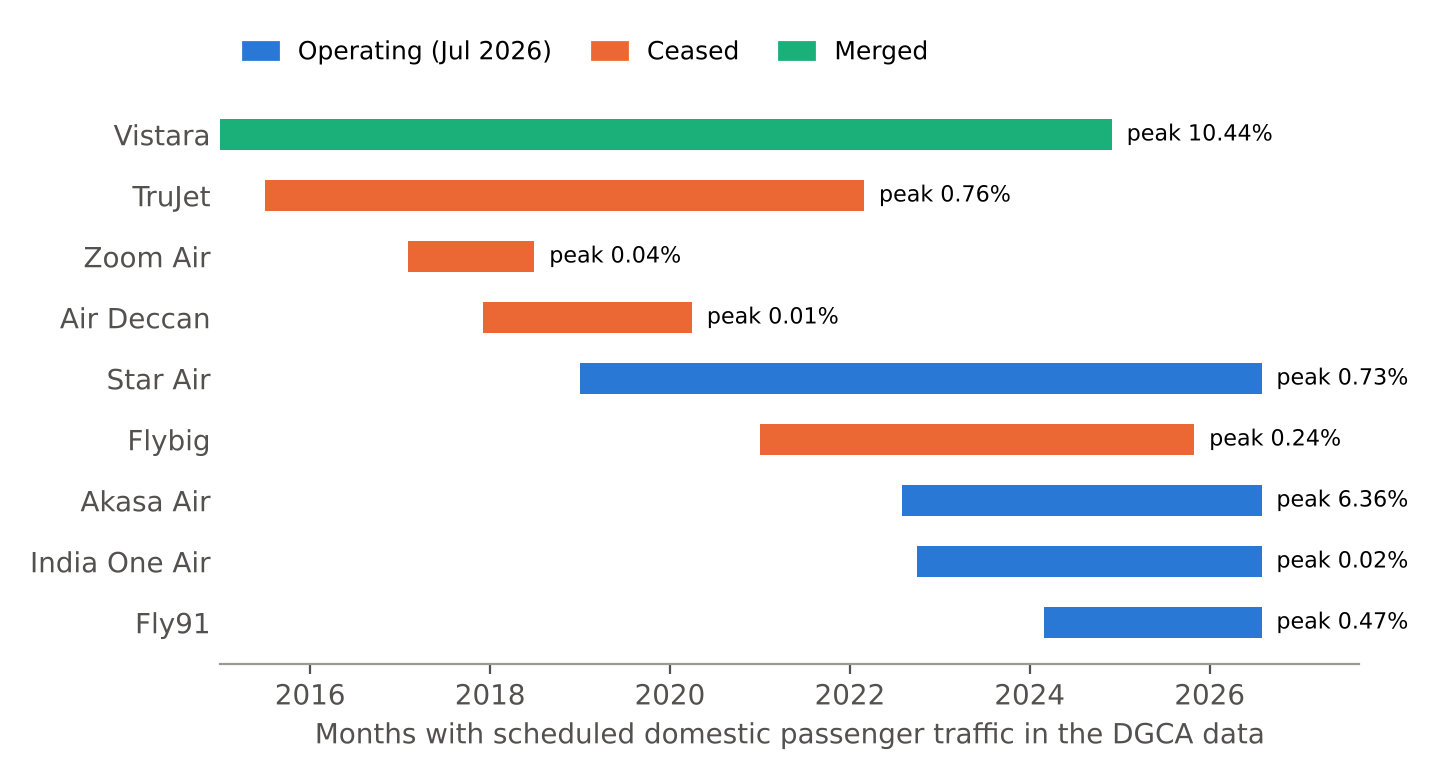
\includegraphics[width=0.92\textwidth]{figures/fig_o3_lifespans.png}
\captionof{figure}{O3: Operating span and peak passenger share of the nine entrants, January 2015--July 2026; colour shows the outcome at July 2026. Source: DGCA via Kubicek (2026); authors' calculations.}
\label{fig:o3-life}
\end{minipage}

\subsubsection{Financial record coverage}
\label{app:eda-financial-coverage}
ICRA (2024, 2026) supplies operating income, after-tax results and funding evidence for Vistara FY2023--24 and Akasa FY2025--26. The December 2025 Lok Sabha reply supplies available FY2023--25 after-tax results; Rajya Sabha (2019, 2021) supplies FY2017--21 operating results. Company/press records supplement funding and outcomes. These are not a balanced panel; provisional figures, revisions, press estimates and accounting bases remain identified below, with missing values never treated as zero.

\begin{minipage}{\textwidth}
\footnotesize
\setlength{\tabcolsep}{3pt}
\captionof{table}{O3: Public financial evidence for the seven regional entrants (Rs crore)}
\label{tab:o3-fy25}
\fontsize{10}{12}\selectfont\setstretch{1}\setlength{\tabcolsep}{3pt}
\renewcommand{\arraystretch}{1.15}
\begin{tabular}{|>{\raggedright\arraybackslash}p{\dimexpr0.12\linewidth-2\tabcolsep-1.1666666666666667\arrayrulewidth\relax}|>{\raggedright\arraybackslash}p{\dimexpr0.15\linewidth-2\tabcolsep-1.1666666666666667\arrayrulewidth\relax}|>{\raggedright\arraybackslash}p{\dimexpr0.15\linewidth-2\tabcolsep-1.1666666666666667\arrayrulewidth\relax}|>{\raggedright\arraybackslash}p{\dimexpr0.12\linewidth-2\tabcolsep-1.1666666666666667\arrayrulewidth\relax}|>{\raggedright\arraybackslash}p{\dimexpr0.15\linewidth-2\tabcolsep-1.1666666666666667\arrayrulewidth\relax}|>{\raggedright\arraybackslash}p{\dimexpr0.31\linewidth-2\tabcolsep-1.1666666666666667\arrayrulewidth\relax}|}
\hline
\textbf{Airline (outcome)} & \textbf{Year} & \textbf{Result} & \textbf{Revenue} & \textbf{Result / revenue (\%)} & \textbf{Basis} \\
\hline
Fly91 (operating) & FY2024; FY2025 & $-31.42$; $-67.65$ & n.a.; 127.4 & n.a.; $-53.1$ & Ministry, after tax, FY2025 provisional; revenue press-reported \\
\hline
Star Air (operating) & FY2023; FY2024; FY2025 & $-20.84$; $-33.31$; $+68.75$ & n.a.; about 360; about 650 & n.a.; about $-9$; about $+11$ & Ministry, after tax, FY2025 provisional; revenue management-reported \\
\hline
India One Air (operating) & FY2023; FY2024; FY2025 & $-8.73$; $-3.23$; $+3.34$ & n.a. & n.a. & Ministry, after tax, FY2025 provisional \\
\hline
Flybig (ceased) & FY2023; FY2024 & $+5.59$; $+4.83$ & n.a. & n.a. & Ministry, after tax; no FY2025 figure \\
\hline
TruJet (ceased) & FY2017, FY2018, FY2019 & $-80.77$; $-85.15$; $-41.00$ & 126.14; 195.68; 265.00 & $-64.0$; $-43.5$; $-15.5$ & Operating result (Rajya Sabha, 2019); FY2019 provisional \\
\hline
TruJet & FY2019, FY2020, FY2021 & $-17.56$; $-10.17$; $-143.16$ & n.a. & n.a. & Operating result (Rajya Sabha, 2021); FY2020--21 provisional \\
\hline
Zoom Air (ceased) & FY2017, FY2018, FY2019 & $+0.14$; $+0.81$; $-1.40$ & 2.61; 17.40; 10.36 & $+5.4$; $+4.7$; $-13.5$ & Operating result (Rajya Sabha, 2019); FY2019 provisional \\
\hline
Air Deccan (ceased) & FY2018, FY2019 & $-13.55$; $-28.90$ & 62.93; 4.70 & $-21.5$; n.m. & Operating result (Rajya Sabha, 2019); may include non-scheduled business \\
\hline
\end{tabular}
\par\raggedright\footnotesize ``n.a.'' means no figure found; ``n.m.'' means not meaningful. Vistara and Akasa Air are in Table~\ref{tab:o3-fin}. Ministry figures are profits or losses after income taxes and extraordinary items. Operating results exclude interest, tax and other non-operating items, so rows on different bases are not comparable. TruJet's FY2019 loss is shown twice because the 2021 reply revises the 2019 provisional figure. Fly91's revenue and Star Air's revenue are press-reported and the underlying filings were not inspected. Sources: Ministry of Civil Aviation (2025); Rajya Sabha (2019, 2021); Whalesbook (2026); Aviation A2Z (2026).
\end{minipage}\par\medskip


\subsubsection{Entrant dates, outcomes and early share milestones}

\par
\begingroup
\flowtablestyle
\fontsize{10}{12}\selectfont
\begin{longtable}{|l|l|l|r|r|l|}
\caption{Entrant observation dates, early passenger shares and outcomes.}\label{tab:detail-o3-summary}\label{tab:o3-outcomes}\\
\hline
\textbf{Airline} & \textbf{First} & \textbf{Last} & \textbf{$\tau=12$ (\%)} & \textbf{$\tau=24$ (\%)} & \textbf{Outcome}\\
\hline
\endfirsthead
\multicolumn{6}{c}{Table~\thetable\ (continued)}\\
\hline
\textbf{Airline} & \textbf{First} & \textbf{Last} & \textbf{$\tau=12$ (\%)} & \textbf{$\tau=24$ (\%)} & \textbf{Outcome}\\
\hline
\endhead
\endfoot
\endlastfoot
Vistara & Jan 2015 & Nov 2024 & 1.97 & 3.27 & Merged\\
\hline
Akasa Air & Aug 2022 & Jul 2026 & 4.24 & 4.51 & Operating\\
\hline
TruJet & Jul 2015 & Feb 2022 & 0.35 & 0.48 & Ceased\\
\hline
Star Air & Jan 2019 & Jul 2026 & 0.09 & 0.20 & Operating\\
\hline
Fly91 & Mar 2024 & Jul 2026 & 0.08 & 0.23 & Operating\\
\hline
Flybig & Jan 2021 & Oct 2025 & 0.11 & 0.17 & Ceased\\
\hline
Zoom Air & Feb 2017 & Jun 2018 & 0.03 & -- & Ceased\\
\hline
India One Air & Oct 2022 & Jul 2026 & 0.01 & 0.02 & Operating\\
\hline
Air Deccan & Dec 2017 & Mar 2020 & -- & -- & Ceased\\*
\noalign{\hrule height\arrayrulewidth\nobreak}
\multicolumn{6}{@{}p{\linewidth}@{}}{\resultstablenotes{$\tau$ counts calendar months from first traffic; dashes mean no observation at that age. Traffic months, peaks and 36-month shares are in Table~\ref{tab:o3-summary}.}{DGCA via Kubicek (2026); outcome sources below.}}\\
\end{longtable}
\endgroup

\textbf{Exclusions and status sources.} Air Pegasus, Air Carnival, Air Odisha, Air Heritage, Pawan Hans and Air Taxi are outside the nine-entrant list; AIX Connect is the AirAsia India rebrand, not new entry. Vistara merged on 12 November 2024; SIA exchanged 49\% of Vistara for 25.1\% of enlarged Air India (Singapore Airlines, 2025; Tata Sons, 2024). Akasa began on 7 August 2022 (Akasa Air, 2025b). Star Air, Fly91 and India One Air appear as operating commuter airlines in the Ministry's December 2024 report, with traffic through July 2026 (Ministry of Civil Aviation, 2025).

TruJet's legal closure is 11 May 2022 after lessor withdrawal; its announced 2025 revival still required permit renewal and has no subsequent traffic here (Ministry of Civil Aviation, 2026; India Seatrade News, 2025). Flybig's final traffic precedes the November 2025 deregistration request and 13 December 2025 AOC closure (Joshi, 2025; Ministry of Civil Aviation, 2026). Zoom suspended in July 2018, after its final June traffic (Business Today, 2019). Air Deccan appears in the Ministry's ceased-operator list (2024). Traffic endpoints are not legal closure dates.


\begin{minipage}{\textwidth}
\centering
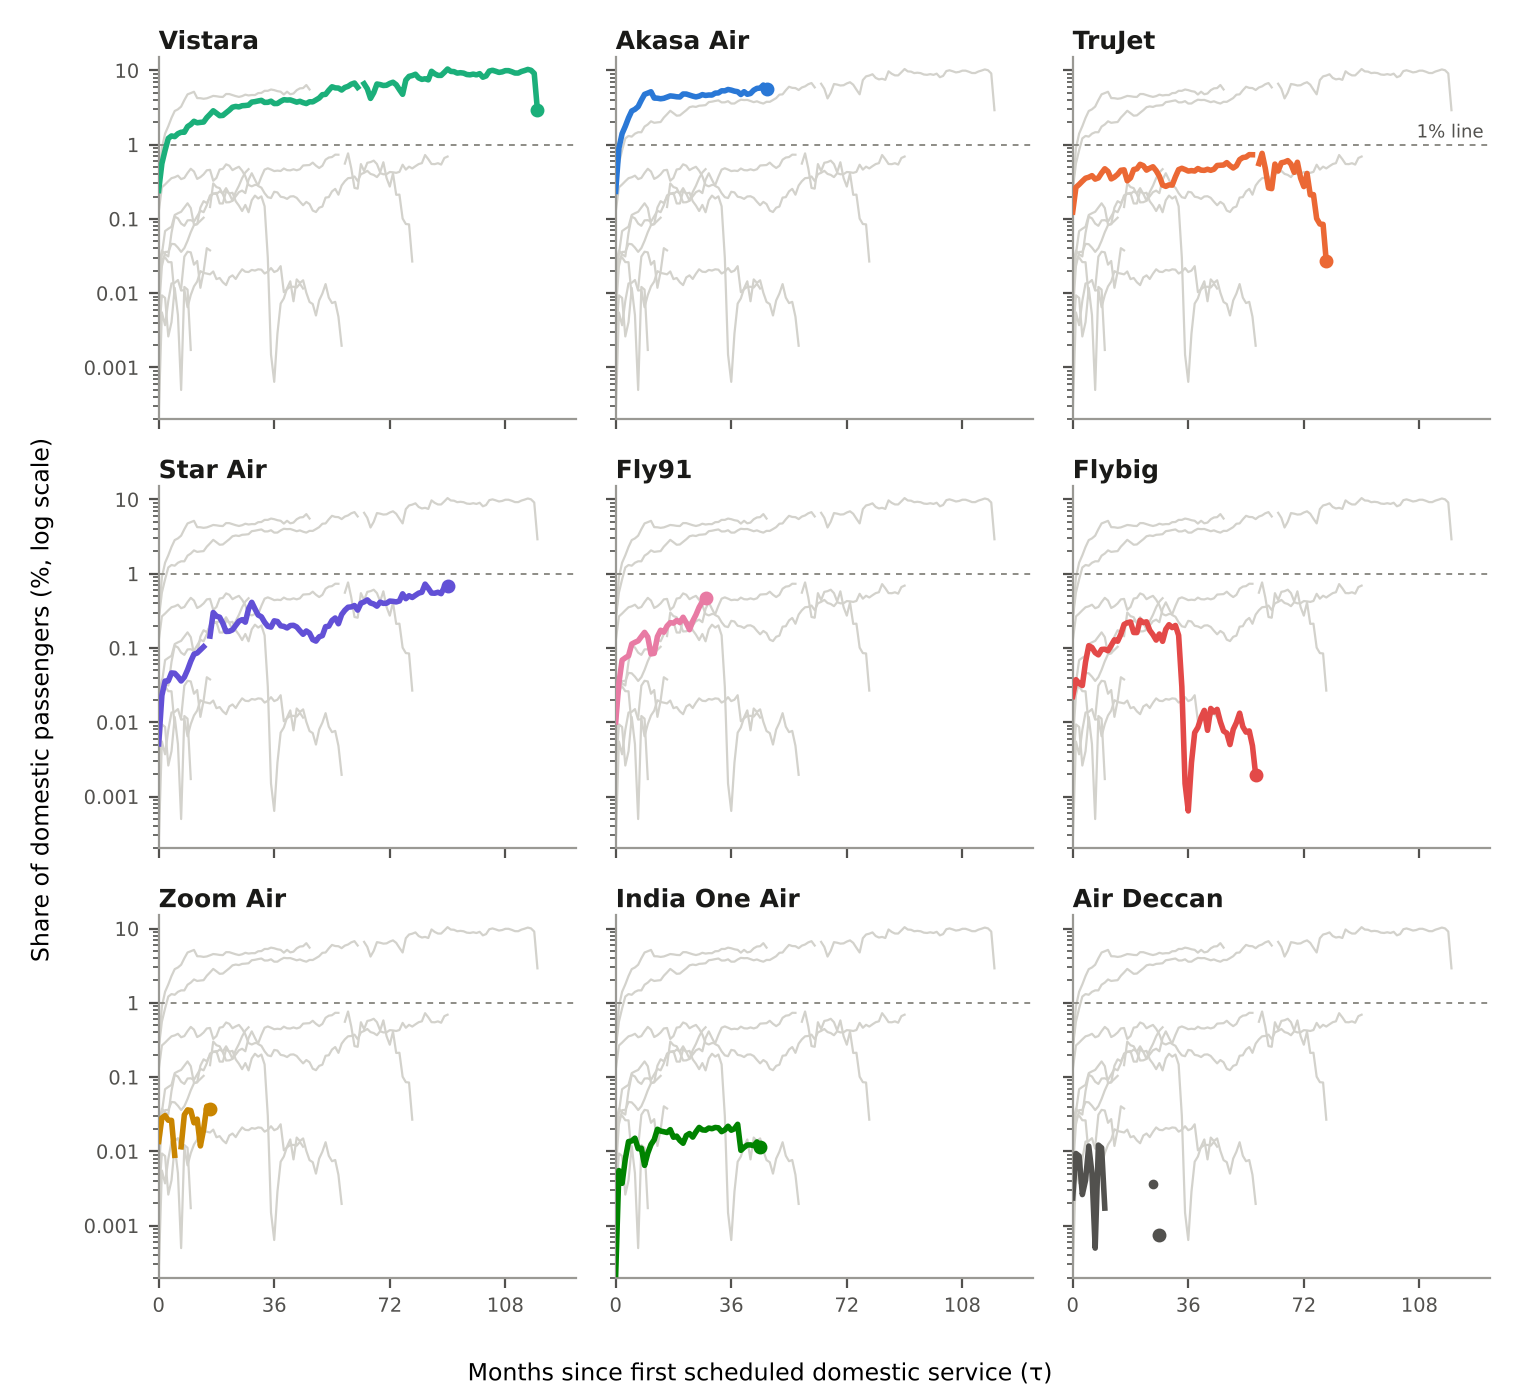
\includegraphics[width=0.82\textwidth]{figures/fig_o3_age.png}
\captionof{figure}{O3: Passenger share of the nine entrants by months since first service (log scale). One panel per entrant (coloured); the other eight are shown in grey for reference, and the dashed line marks 1\%. Each line ends at the airline's last observed month; gaps are months missing from the data (April 2020 for Vistara, TruJet and Star Air). Shares below 0.0002\% are drawn at the axis floor, and Vistara's last point (November 2024) is a partial month. Source: DGCA via Kubicek (2026); authors' calculations.}
\label{fig:o3-age}
\end{minipage}

\subsubsection{Seasonal route inputs and calculation}

\begingroup
\renewcommand{\theHequation}{review-o3-season-departures}
\textbf{Full-season counts.} Sum deduplicated services across both directions, counting only valid dates and operating weekdays within the chosen season:
\begin{equation}
D_{a,r,s}=\sum_{j\in(a,r)}\ \sum_{d\in s}
\mathbf{1}\{b_j\leq d\leq e_j\}\,
\mathbf{1}\{\mathrm{weekday}(d)\in W_j\}.
\tag{O3.1}\label{eq:o3-season-departures}
\end{equation}
Here $a,r,s$ denote airline, pair and season; $b_j,e_j,W_j$ are service $j$'s validity dates and weekdays. These are scheduled departures, not verified operations.
\renewcommand{\theHequation}{review-o3-season-share}
\begin{equation}
\mathrm{SeasonShare}_{a,r,s}=100\,
\frac{D_{a,r,s}}{\sum_b D_{b,r,s}}.
\tag{O3.2}\label{eq:o3-season-share}
\end{equation}
The denominator includes all recorded airlines on that pair and season. Sole-operator and at-least-50\% flags use this share; entrants' seasons differ, not a common-date comparison. For example, regional entrants have 75 sole-operator records out of 109, giving $100(75/109)=68.8\%$; ceased entrants have $100(32/50)=64.0\%$. Units are airline--pair--season records, not unique airports. TruJet's separate November 2019 result is 17 of 22 pairs.
\endgroup
\par


\par
\begingroup
\flowtablestyle
\fontsize{10}{12}\selectfont
\begin{longtable}{|>{\raggedright\arraybackslash}p{\dimexpr0.2\linewidth-2\tabcolsep-1.2\arrayrulewidth\relax}|>{\raggedright\arraybackslash}p{\dimexpr0.21\linewidth-2\tabcolsep-1.2\arrayrulewidth\relax}|>{\raggedright\arraybackslash}p{\dimexpr0.2\linewidth-2\tabcolsep-1.2\arrayrulewidth\relax}|>{\raggedright\arraybackslash}p{\dimexpr0.2\linewidth-2\tabcolsep-1.2\arrayrulewidth\relax}|>{\raggedright\arraybackslash}p{\dimexpr0.19\linewidth-2\tabcolsep-1.2\arrayrulewidth\relax}|}
\caption{Additional inputs for the full-season route comparisons.}\label{tab:o3-routes}\\
\hline
\textbf{Airline} & \textbf{Season} & \textbf{Scheduled departures} & \textbf{Median route share (\%)} & \textbf{Airlines with filings}\\
\hline
\endfirsthead
\multicolumn{5}{c}{Table~\thetable\ (continued)}\\
\hline
\textbf{Airline} & \textbf{Season} & \textbf{Scheduled departures} & \textbf{Median route share (\%)} & \textbf{Airlines with filings}\\
\hline
\endhead
\endfoot
\endlastfoot
Vistara & Winter 2023 & 43,523 & 20.3 & 9\\
\hline
Akasa Air & Summer 2026 & 32,340 & 22.8 & 9\\
\hline
TruJet & Winter 2021 & 9,463 & 100.0 & 10\\
\hline
Star Air & Summer 2026 & 11,589 & 100.0 & 9\\
\hline
Fly91 & Summer 2026 & 7,503 & 100.0 & 9\\
\hline
Flybig & Summer 2022 & 4,894 & 100.0 & 9\\
\hline
Zoom Air & Winter 2017 & 588 & 66.7 & 11\\
\hline
India One Air & Summer 2026 & 3,777 & 100.0 & 9\\
\hline
Air Deccan & Winter 2019 & 1,188 & 100.0 & 11\\*
\noalign{\hrule height\arrayrulewidth\nobreak}
\multicolumn{5}{@{}p{\linewidth}@{}}{\resultstablenotes{Airport-pair, sole-operator and at-least-50\% counts are in Table~\ref{tab:results-o3-route-summary}. Departures pool both directions over the full selected season. Median shares are across the entrant's airport pairs. The last column counts airlines with recorded filings in that season. Seasons differ across entrants.}{DGCA approved domestic schedules; authors' calculations.}}\\
\end{longtable}
\endgroup


\textbf{Separate monthly example.} In November 2019, TruJet supplied all 60 recorded scheduled flights on Chennai--Salem, giving a 100\% frequency share and HHI of 10,000. The airport pair carried 3,281 passengers across all airlines, while TruJet's national passenger share was 0.63\%. This monthly example is separate from the seasonal totals.

\Needspace{8\baselineskip}
\subsubsection{Financial inputs and worked ratios}

\par
\begingroup
\flowtablestyle
\fontsize{10}{12}\selectfont
\begin{longtable}{|>{\raggedright\arraybackslash}p{\dimexpr0.26\linewidth-2\tabcolsep-1.3333333333333333\arrayrulewidth\relax}|>{\raggedright\arraybackslash}p{\dimexpr0.37\linewidth-2\tabcolsep-1.3333333333333333\arrayrulewidth\relax}|>{\raggedright\arraybackslash}p{\dimexpr0.37\linewidth-2\tabcolsep-1.3333333333333333\arrayrulewidth\relax}|}
\caption{Revenue, profit and funding inputs for Vistara and Akasa Air.}\label{tab:detail-o3-fin}\\
\hline
\textbf{Input} & \textbf{Vistara (FY2023$\to$FY2024)} & \textbf{Akasa Air (FY2025$\to$FY2026)}\\
\hline
\endfirsthead
\multicolumn{3}{c}{Table~\thetable\ (continued)}\\
\hline
\textbf{Input} & \textbf{Vistara (FY2023$\to$FY2024)} & \textbf{Akasa Air (FY2025$\to$FY2026)}\\
\hline
\endhead
\endfoot
\endlastfoot
Operating income (Rs crore) & 12,261.4 $\to$ 15,310.3 & 4,582.7 $\to$ 6,167.9\\
\hline
Profit after tax (Rs crore) & $-1{,}393.3\to-581.1$ & $-1{,}983.5\to-2{,}716.0$\\
\hline
Funding & Rs~10,020 crore from Tata and Singapore Airlines by Aug 2024 & Equity round completed 19 Aug 2025; about US\$125 million is a press estimate\\*
\noalign{\hrule height\arrayrulewidth\nobreak}
\multicolumn{3}{@{}p{\linewidth}@{}}{\resultstablenotes{Revenue and profit after tax are in Rs crore. Company figures include domestic and international operations. Funding amounts retain their reported currency. The US\$125 million figure is a press estimate. Calculated growth rates and margins are in Table~\ref{tab:o3-fin}.}{ICRA (2024, 2026), Tata and Singapore Airlines company records, and the O3 source records.}}\\
\end{longtable}
\endgroup



For Vistara, the figures above give
\begin{align*}
\mathrm{Revenue\ growth}
&=100\frac{15{,}310.3-12{,}261.4}{12{,}261.4}\approx24.87\%,\\
\mathrm{FY2024\ net\ margin}
&=100\frac{-581.1}{15{,}310.3}\approx-3.80\%.
\end{align*}
The same calculations give Akasa Air's revenue growth and net margins in Table~\ref{tab:o3-fin}.
Earlier regional financial records and accounting qualifications are in Table~\ref{tab:o3-fy25}.
\end{mergedcontribution}
\subsection{O4: Route coverage, sensitivity and unused capacity}
\label{app:o4-route-preparation}
\begin{mergedcontribution}{authorGoutham}
Common concentration measures and aggregation follow Appendix~\ref{app:shared-calculations}. Named IndiGo and Air India Group frequency shares use the same route denominator; their signed difference (IndiGo minus Air India Group) is retained in the focus-period CSV and can be negative. Capacity-buffer definitions and workings are given in Appendix~\ref{app:o4-capacity-buffer}.

\subsubsection{O4: Flags, coverage and missingness}
\label{app:o4-flags}
Concentration flags use ownership HHI $>1{,}800$ \parencite[Section~2.1]{dojftc2023merger}, CR2 $\geq80\%$, gap $>20$ pp and fringe $\leq20\%$. The gap and IndiGo-exposure ($\geq60\%$ of flights) cut-offs are study-defined; IndiGo-only requires 100\%. H5 requires the IndiGo--Air India leading pair, CR2 and gap conditions; H6 uses HHI alone. The route joint flag requires a unique pair, and its IndiGo-led variant also requires IndiGo first. These describe concentration, not pricing conduct.

A rank-two/three tie prevents a unique leading pair; a two-way first-place tie alone does not. Unique leadership requires strictly exceeding every rival; first-place ties are counted separately, with alphabetical order used only for display. Missing/excluded observations are omitted and shown grey in the heatmap, never imputed as zero. Observed zero gaps, fringe shares and exposure counts remain valid. Source-quality and capacity-validity rules are below.

\subsubsection{National condition checks}
\label{app:o4-national-summary}
H5 holds in $48/138=34.8\%$ of observed months and $20/20=100\%$ during December 2024--July 2026; HHI exceeds 1,800 in all 138 months. April 2020 is missing. In the focus period, HHI ranges from 4,468.57 to 5,144.35 and fringe share from 8.30\% to 10.87\%. These are not independent tests: fringe is $100-\mathrm{CR2}$, and CR2 $\geq80\%$ implies $s_1^2+s_2^2\geq(s_1+s_2)^2/2\geq3{,}200$. See Table~\ref{tab:o4-national-results}.

The second-largest group is Jet (January 2015--January 2019), SpiceJet (February 2019--April 2021), Air India (May--August 2021), Vistara (September 2021), Go First (October--December 2021) and Air India Group (January 2022 onward), using the passenger series in Figure~\ref{fig:o4-national-eda}.

\subsubsection{Route samples and concentration over time}
\label{app:eda-route-support}
Table~\ref{tab:review-route-samples} separates overlapping samples from recovered DGCA schedules. Directions are pooled; O3 uses brands, O4 ownership groups. Counts with different units are not added.

\begin{resultstable}{Samples drawn from the DGCA schedule archive.}{tab:review-route-samples}
\color{black}
\begin{tabular}{|>{\raggedright\arraybackslash}p{\dimexpr0.31\linewidth-2\tabcolsep-1.5\arrayrulewidth\relax}|>{\raggedright\arraybackslash}p{\dimexpr0.69\linewidth-2\tabcolsep-1.5\arrayrulewidth\relax}|}
\hline
\textbf{Sample} & \textbf{Coverage and observation unit} \\
\hline
Entrant full-season & Nine entrants; 229 airline--pair--season observations; all scheduled departures in each selected season \\
\hline
Entrant major routes & 20 pairs, April 2019--July 2026; airline--pair--month \\
\hline
TruJet regional extension & 30 pairs, 14 observed months in 2019--2022; airline--pair--month \\
\hline
Ownership concentration & 20 fixed pairs; 1,150 pair--months across 66 available months, April 2019--September 2026 \\
\hline
\end{tabular}
\par\vspace{5pt}{\footnotesize\setstretch{1.05}\raggedright \textbf{Note:} Entrants use the latest usable season before closure/merger or latest available season. O4's fixed top 20 and nested top ten use 2025 passenger totals.\par\textbf{Source:} Sweta\textquotesingle s and Goutham\textquotesingle s DGCA schedule preparation.\par}
\end{resultstable}
Figure~\ref{fig:o4-route-heatmap} uses a common 0--10,000 scale; grey cells are missing, not interpolated.

\begin{figure}[H]
\centering
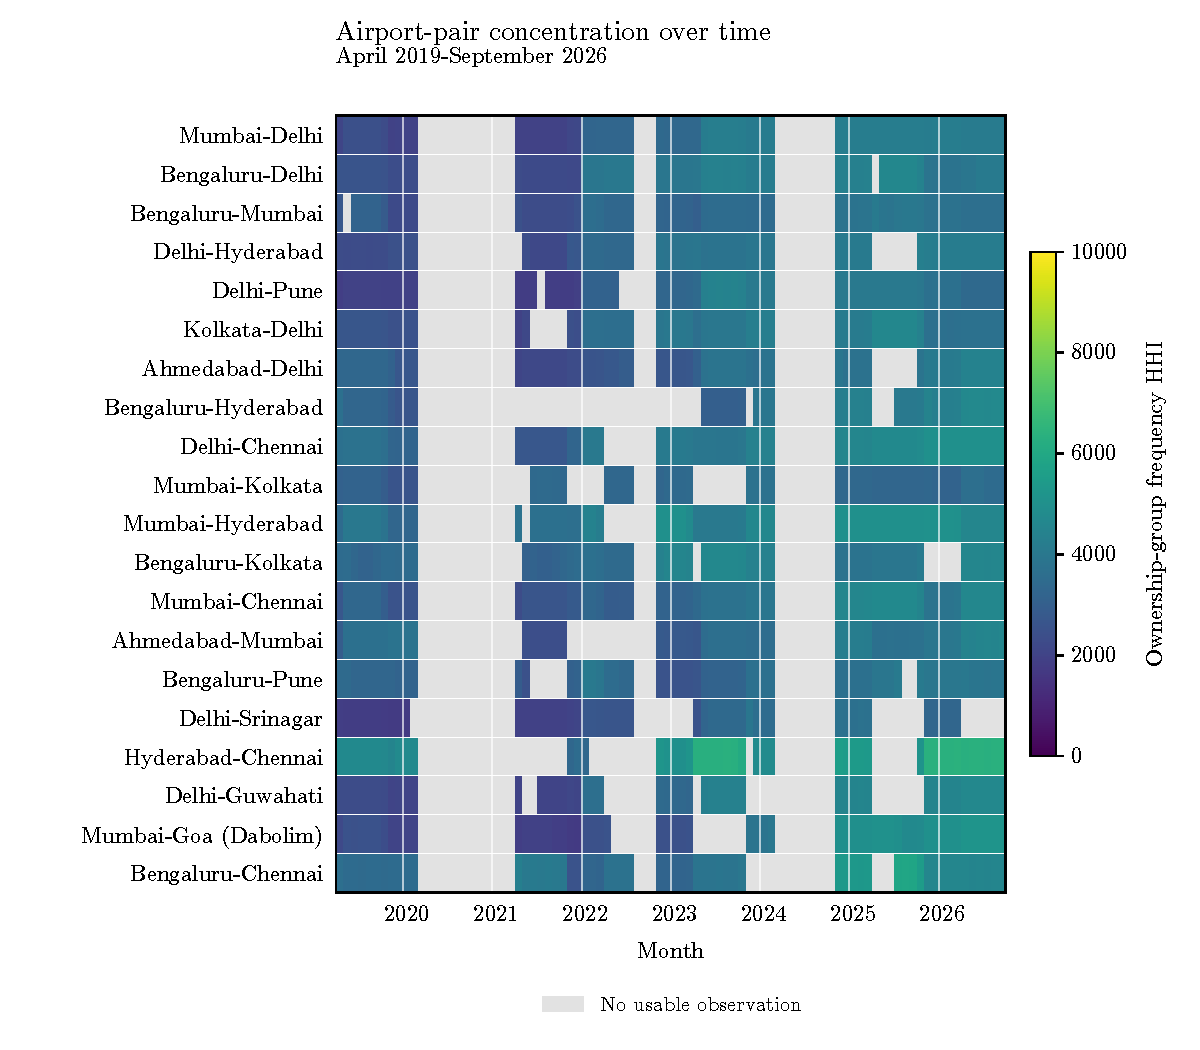
\includegraphics[width=\linewidth]{figures/o4_route_hhi_heatmap.pdf}
\caption{Ownership-group frequency HHI by airport pair and month.}
\label{fig:o4-route-heatmap}
\vspace{2pt}
\begin{minipage}{\linewidth}
\footnotesize\setstretch{1.1}
\textit{Source:} DGCA approved domestic schedules; authors' calculations.
\end{minipage}
\end{figure}

\subsubsection{O4: Route concentration calculations}
\label{app:o4-route-calculations}
\textbf{Delhi--Pune, June 2026.} Prepared DGCA schedules give Air India Group $618=472+146$ flights, IndiGo 524, SpiceJet 168 and Akasa 120, totalling 1,430. Applying Appendix~\ref{app:shared-calculations} without rounding intermediate shares,
\[
\begin{aligned}
\HHI&=10{,}000\frac{618^2+524^2+168^2+120^2}{1{,}430^2}\approx3{,}418.87,\\
\mathrm{CR2}&=100\frac{618+524}{1{,}430}\approx79.8601\%.
\end{aligned}
\]
The gap is 6.5734 pp, fringe 20.1399\% and IndiGo share 36.6434\%. Air India leads: this contributes to H6 and the unique pair, but not the CR2, gap or IndiGo-exposure flags. Pooled condition percentages use retained pair-months; monthly percentages use that month's available pairs, not a constant 20.

\Needspace{4\baselineskip}
\subsubsection{O4: Route subset comparisons and leading pairs}
\label{app:o4-route-checks}
Of 1,150 observations, CR2 is at least 80\% in 583 (50.70\%) and the gap exceeds 20 pp in 368 (32.00\%). The unique IndiGo--Air India pair occurs in 730 (63.48\%); rank-two/three ties prevent pair identification in 58 (5.04\%), without changing concentration measures. Conditions overlap; counts are not added.

Full-period medians are CR2 80.00\%, gap 13.73 pp, fringe 20.00\% and IndiGo frequency share 43.60\%. The 79 observations meeting the IndiGo $\geq60\%$ flag occur on Bengaluru--Kolkata, Chennai--Hyderabad and Bengaluru--Chennai. Monthly exposure ranges from 0\% to 11.11\% of available airport pairs. In December 2025, Chennai--Hyderabad is the only one of 19 available airport pairs meeting the flag, with IndiGo at 78.10\%.

Table~\ref{tab:o4-route-sensitivity} compares overlapping subsets, not additive samples. Exact endpoint agreement does not prove complete airline filings.

\begin{minipage}{\linewidth}
\captionsetup{font=small,labelfont=bf,justification=raggedright,singlelinecheck=false,hypcap=false}
\captionof{table}{Route concentration and IndiGo exposure across sample definitions.}
\label{tab:o4-route-sensitivity}
\centering
{\small\setstretch{1.1}\setlength{\tabcolsep}{4pt}\fontsize{10}{12}\selectfont\setstretch{1}\setlength{\tabcolsep}{3pt}
\renewcommand{\arraystretch}{1.15}
\begin{tabular}{|>{\raggedright\arraybackslash}p{\dimexpr0.4\linewidth-2\tabcolsep-1.25\arrayrulewidth\relax}|>{\raggedright\arraybackslash}p{\dimexpr0.2\linewidth-2\tabcolsep-1.25\arrayrulewidth\relax}|>{\raggedright\arraybackslash}p{\dimexpr0.2\linewidth-2\tabcolsep-1.25\arrayrulewidth\relax}|>{\raggedright\arraybackslash}p{\dimexpr0.2\linewidth-2\tabcolsep-1.25\arrayrulewidth\relax}|}
\hline
\textbf{Sample} & \textbf{$N$} & \textbf{HHI $>1{,}800$: $n$ (\%)} & \textbf{IndiGo $\geq60\%$: $n$ (\%)} \\
\hline
Full sample & 1,150 & 1,143 (99.39\%) & 79 (6.87\%) \\
\hline
Exact endpoint matches & 303 & 301 (99.34\%) & 26 (8.58\%) \\
\hline
December 2025 & 19 & 19 (100.00\%) & 1 (5.26\%) \\
\hline
\end{tabular}
\par}
\vspace{4pt}
{\footnotesize\setstretch{1.1}\raggedright\textit{Note:} $N$ is retained airport-pair/month observations and $n$ is observations meeting each condition. Exact matches and December 2025 are subsets of April 2019--September 2026. No subset contains an IndiGo-only observation.\par
\textit{Source:} DGCA approved domestic schedules; authors' calculations.\par}
\end{minipage}

\subsubsection{O4: Matched focus-period calculations and coverage}
\label{app:o4-route-focus}
December 2024--July 2026 retains 184/200 top-ten and 350/400 top-20 pair-months, covering all 20 months. Monthly coverage ranges from 6--10 and 12--20 pairs respectively: both are complete through March 2025, lowest in April (6/12), and 10/19 from November 2025 onward. Ranking and screening stay fixed.

National medians use 20 months; route medians use 184 or 350 equally weighted pair-months (Appendix~\ref{app:shared-calculations}). Pairs with more retained months contribute more observations; there is no volume weighting or pooling of flight totals.

IndiGo-led joint shares are $100(9/184)=4.89\%$ for the top ten and $100(50/350)=14.29\%$ for the top 20, requiring the unique pair, CR2 $\geq80\%$, gap $>20$ pp and IndiGo first.
First-place ties are counted separately: IndiGo leads in 86, Air India in 94 and both tie in four top-10 observations; the corresponding top-20 counts are 214, 132 and four. IndiGo supplies at least 60\% of scheduled flights in 26 of 350 top-20 observations and none of the 184 top-ten observations. Neither focus-period sample contains an IndiGo-only observation.

\subsubsection{O4: Capacity-buffer calculations}
\label{app:o4-capacity-buffer}
Let $I$ denote IndiGo and $j$ a retained rival airline brand. For month $t$, unused rival capacity $U_t$ and the buffer percentage $B_t$ are
\[
U_t=\sum_{j\ne I}(\mathrm{ASK}_{jt}-\mathrm{RPK}_{jt}),
\qquad B_t=100\frac{U_t}{\mathrm{RPK}_{It}}.
\]
Each rival brand is counted once; the denominator is all IndiGo RPK, not rivals' ASK or cancellation-affected traffic. The 19 selected records satisfy ASK $>0$ and $0\leq\mathrm{RPK}\leq\mathrm{ASK}$. Table~\ref{tab:o4-capacity-inputs} gives the aggregate inputs in billions (source conversion: Appendix~\ref{app:shared-calculations}).

\begin{minipage}{\linewidth}
\captionsetup{font=small,labelfont=bf,justification=raggedright,singlelinecheck=false,hypcap=false}
\captionof{table}{Capacity-buffer inputs, December 2024 and December 2025 (billions).}
\label{tab:o4-capacity-inputs}
\centering
{\small\setstretch{1.1}\fontsize{10}{12}\selectfont\setstretch{1}\setlength{\tabcolsep}{3pt}
\renewcommand{\arraystretch}{1.15}
\begin{tabular}{|>{\raggedright\arraybackslash}p{\dimexpr0.48\linewidth-2\tabcolsep-1.3333333333333333\arrayrulewidth\relax}|>{\raggedright\arraybackslash}p{\dimexpr0.26\linewidth-2\tabcolsep-1.3333333333333333\arrayrulewidth\relax}|>{\raggedright\arraybackslash}p{\dimexpr0.26\linewidth-2\tabcolsep-1.3333333333333333\arrayrulewidth\relax}|}
\hline
\textbf{Input} & \textbf{Dec 2024} & \textbf{Dec 2025} \\
\hline
Rivals' ASK & 6.384761131 & 6.618678370 \\
\hline
Rivals' RPK & 5.492545663 & 5.946741054 \\
\hline
IndiGo RPK & 9.113052 & 8.207875 \\
\hline
\end{tabular}
\par}
\vspace{4pt}
{\footnotesize\setstretch{1.1}\raggedright\textit{Note:} Rival sums exclude IndiGo. Flybig has no retained positive-passenger record in December 2025; absence is not an imputed zero.\par
\textit{Source:} DGCA monthly airline traffic via Kubicek (2026); authors' calculations.\par}
\end{minipage}

Substituting the table inputs gives
\begin{align*}
B_{2024}&=100\frac{6.384761131-5.492545663}{9.113052}\approx9.7905\%,\\
B_{2025}&=100\frac{6.618678370-5.946741054}{8.207875}\approx8.1865\%.
\end{align*}
Thus $\Delta B=-1.6040$ pp; $U$ falls from 0.892215468 to 0.671937316 billion seat-km, or $100(U_{2025}/U_{2024}-1)=-24.69\%$. CSVs retain airline inputs and unrounded aggregates.

\textbf{Capacity preparation.} Ten brands in December 2024 and nine in December 2025 pass the common filter and capacity-validity screen. The two historical zero-ASK/RPK records in Appendix~\ref{app:o1-cleaning} remain flagged, not imputed; neither enters this comparison.

\textbf{O4 route preparation.} The archive contains 228 DGCA schedule PDFs; 92 contribute departure rows to the retained sample. Extraction preserves PDF, page and row references. Flight weekdays and validity dates are expanded into calendar dates, duplicate flight-date-directed legs are removed, and directions are pooled before shares are calculated. The top 20 pairs are selected using 2025 passenger totals from the \href{https://github.com/mkubicek/india-aviation-stats/tree/16770ac59dae61ce7b80fd8bd67dd7f4cef280a6}{DGCA-derived dataset distributed by Kubicek (2026)}.

The screen requires full-month coverage, endpoint discrepancy $100\sum_a|D_a-A_a|/\sum_aD_a\leq5\%$ (departures $D$, arrivals $A$, pooled directions), and ten retained pairs per month. Exact match requires $D_a=A_a$ for every airline. Excluding Chennai--Hyderabad in February--March 2022, where TruJet's plan extends beyond suspension, reduces 1,152 to 1,150 observations; 303 match exactly. Missing filings can escape the screen: these are recovered approved schedules, not actual operations or passenger shares.
\end{mergedcontribution}
\section{Reproduction}
\label{app:reproduction}
\textbf{O1, O2 and O4.} From the \href{https://github.com/Goutham7358/Assignment3_Code}{code repository} root, use Python 3.10+ and the included prepared O4 inputs. Raw snapshot/version/fingerprint: \path{data/raw/carrier_monthly.csv} and \path{data/SOURCE.md}; O4 inputs: \path{data/processed/} and \path{data/processed/routes/}. Schedule provenance/rebuilding: \path{data/ROUTE_SOURCES.md} and \path{data/source/}.
\begingroup
\footnotesize
\begin{verbatim}
python3 -m venv .venv
source .venv/bin/activate
python3 -m pip install -r requirements.txt -r O2/requirements.txt
python3 -m pip install pandas statsmodels
python3 O1/data_cleansing.py
python3 O1/HHI_Index_calculation.py
python3 O1/export_results_tables.py
python3 O2/run_analysis.py
python3 O4/EDA/generate_figures.py
python3 O4/Main_Analysis/national_concentration.py
python3 O4/Main_Analysis/route_concentration.py
python3 O4/Main_Analysis/route_focus_period.py
python3 O4/Main_Analysis/capacity_buffer.py
python3 O4/Main_Analysis/hypothesis_summary.py
\end{verbatim}
\endgroup
O1 writes \path{data/processed/}, \path{O1/results/} and \path{O1/figures/}; O2/O4 write their \path{output/} directories. Optional O4 input rebuilds use \path{data/source/prepare_national.py} and \path{data/source/prepare_capacity.py}; routes also require archived PDFs and the documented extraction workflow.

\textbf{O3.} In the separate \href{https://github.com/Goutham7358/Economics_New_Entrants_India_Domestic_Aviation}{case-study repository}, follow its input layout: \path{o3_entrant_analysis.py} produces national/event-time results and figures; \path{o3_route_fullseason.py} produces seasonal route counts. Financial sources and accounting bases remain in Appendix~\ref{app:o3-support}; tools disclosure follows this appendix.
